\chapter{微服务架构与跨数据链协议互操作系统设计}

本章基于MIL-STD-6016战术数据链信息标准,设计并实现微服务架构的跨协议互操作系统。系统架构采用四层分层设计,通过微服务模块化实现多标准信息模型的自动导入、语义对齐与协议转换。本章依次阐述系统总体架构、微服务实现、数据模型设计、跨协议互操作架构以及自动化导入系统。

\section{系统总体架构设计}

\subsection{设计目标与总体思路}

系统以MIL-STD-6016战术数据链信息标准为核心,采用微服务架构构建跨协议互操作平台。设计目标包括:多源标准语义互操作、模块化弹性部署、自动化数据处理。

多源标准语义互操作要求系统支持MIL-STD-6016、STANAG 5516、MIL-STD-6020、MQTT、MAVLink等协议的语义对齐。通过统一语义模型和概念映射机制,实现跨标准数据的准确转换,保障不同协议间的语义一致性。

模块化弹性部署通过微服务架构将复杂系统拆分为独立服务模块。每个服务专注特定业务功能,支持独立开发、测试、部署和扩展,提高系统的可维护性、可扩展性和容错能力。

自动化数据处理实现标准化文档的自动识别、结构化提取和协议转换。系统减少人工干预,提高数据处理效率和准确性,支持战术数据链信息处理的自动化。

\subsection{微服务架构理念与原则}

系统采用"高内聚、低耦合、自治服务"的设计理念,遵循四个核心原则:服务拆分、服务治理、数据管理、通信机制。

服务拆分按业务域划分,确保每个微服务具有单一职责和独立演化能力。微服务专注特定业务功能,具有清晰边界,通过标准化API接口通信,避免紧耦合依赖。

服务治理包含注册发现、配置中心、监控与熔断机制。服务注册中心实现自动发现和负载均衡,配置中心支持统一管理和动态更新,监控系统提供健康状态监控和性能分析。

数据管理采用数据库分离与分布式事务一致性保障。每个微服务拥有独立数据库,通过事件驱动和Saga模式保证分布式事务一致性,避免数据耦合和单点故障。

通信机制结合同步(REST/gRPC)与异步(消息队列)模式。实时性要求高的场景采用同步通信,批量处理和事件通知采用异步通信,优化通信效率与系统性能。

\subsection{架构总体分层}

系统整体采用四层分层架构,如图\ref{fig:system_architecture}所示:

\begin{figure}[H]
    \centering
    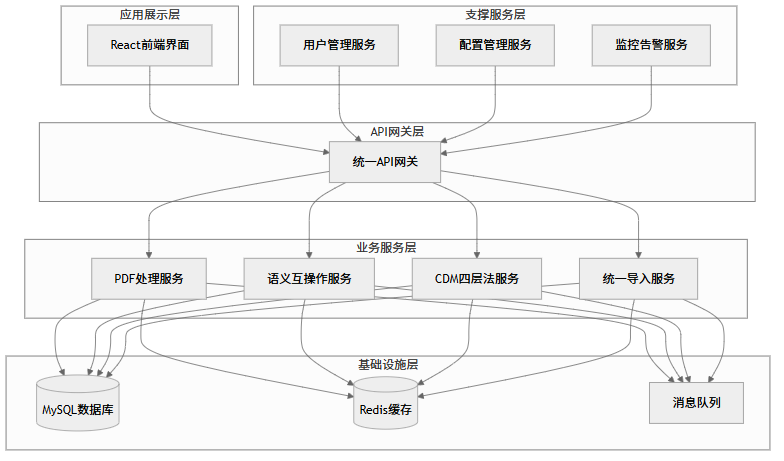
\includegraphics[width=0.9\textwidth]{chapters/fig-0/system_architecture_simple.png}
    \caption{系统总体架构分层图}
    \label{fig:system_architecture}
\end{figure}

API网关层作为系统统一入口,提供请求路由、认证鉴权、访问控制、限流熔断与监控统计功能。该层接收外部请求,执行身份验证、权限检查、请求路由和响应聚合,通过限流和熔断机制保护后端服务。

业务服务层包含PDF解析、语义互操作、CDM四层法、统一导入等核心业务模块。每个服务作为独立业务单元,支持独立开发、测试和部署,体现微服务架构的模块化设计理念。

支撑服务层提供用户配置管理、监控告警、文件日志等系统支持功能。该层包括用户认证、配置管理、监控告警、文件存储等关键功能,构成系统运行的基础保障体系。

基础设施层包含服务注册发现(Consul/Kubernetes)、消息队列(RabbitMQ/Redis)、数据库与缓存集群等核心组件。该层实现服务发现、消息传递、数据存储和缓存等基础功能,为微服务架构提供技术支撑。

\section{微服务架构设计与实现}

\subsection{技术栈与基础组件选型}

系统采用现代化的技术栈,确保高性能、高可用性和可扩展性。技术选型如表\ref{table:tech_stack}所示:

\begin{table}[H]
    \caption{技术栈与基础组件选型}
    \label{table:tech_stack}
    \centering
    \begin{tabular}{|l|l|}
        \hline
        \textbf{功能} & \textbf{技术栈} \\
        \hline
        服务框架 & FastAPI + Python 3.10(高性能异步框架) \\
        服务发现 & Consul + Kubernetes DNS \\
        配置管理 & Consul KV + ConfigMap \\
        消息队列 & RabbitMQ + Redis Pub/Sub \\
        数据存储 & MySQL 8.0 + Redis \\
        监控体系 & Prometheus + Grafana + Jaeger \\
        \hline
    \end{tabular}
\end{table}

服务框架选择FastAPI作为主要框架,利用Python 3.10的异步特性提供高性能API服务。FastAPI具备自动API文档生成、数据验证、类型提示等特性,提高开发效率。

服务发现机制使用Consul作为注册发现中心,支持多数据中心部署和服务健康检查。在Kubernetes环境中,结合Kubernetes DNS实现服务自动发现和负载均衡,形成灵活可靠的服务治理体系。

消息传递采用RabbitMQ作为主要消息队列,提供可靠的消息传递和事务支持,同时使用Redis Pub/Sub进行实时通知和轻量级消息传递。混合消息传递机制保证关键业务数据的可靠性,满足实时通信的性能要求。

数据存储采用MySQL 8.0作为主数据库,利用其ACID事务、JSON数据类型、窗口函数等高级特性,同时使用Redis作为缓存层,提供高性能的数据访问和会话存储。分层存储架构保证数据一致性,提升系统整体性能。

\subsection{微服务模块划分与职责}

系统共包含五类核心服务,每个服务都有明确的职责和边界,如表\ref{table:microservices}所示:

\begin{table}[H]
    \caption{微服务模块划分与职责}
    \label{table:microservices}
    \centering
    \begin{tabular}{|l|l|}
        \hline
        \textbf{模块} & \textbf{核心职责} \\
        \hline
        pdf-service & 自动化标准文档解析与结构化导入 \\
        semantic-service & 跨标准语义分析与字段映射 \\
        cdm-service & CDM四层语义互操作(语义层/映射层/校验层/运行层) \\
        import-service & 多格式文件识别、清洗与批量导入 \\
        api-gateway & 统一接口访问控制、负载均衡、服务监控 \\
        \hline
    \end{tabular}
\end{table}

(1)pdf-service:负责自动化标准文档解析与结构化导入。服务处理MIL-STD-6016、STANAG 5516等标准文档,自动提取消息定义、字段信息和约束条件,转换为结构化数据格式。

(2)semantic-service:实现跨标准语义分析与字段映射。服务提供语义分析引擎,识别不同标准中的语义概念,建立概念间映射关系,支持人工标注和规则学习。

(3)cdm-service:实现CDM四层语义互操作。服务基于Common Data Model四层架构,提供语义层、映射层、校验层和运行层的完整实现,支持不同协议间的语义级转换。

(4)import-service:负责多格式文件识别、清洗与批量导入。服务支持PDF、Excel、XML、JSON等多种格式的文件处理,提供格式自动识别、数据清洗和批量导入功能。

(5)api-gateway:提供统一接口访问控制、负载均衡、服务监控。服务作为系统统一入口,负责请求路由、身份验证、权限控制、限流熔断和监控统计。

\subsection{微服务通信机制}

微服务间的通信采用多种模式,根据业务场景选择合适的通信方式,形成了灵活高效的通信架构。

同步通信使用REST API、gRPC、GraphQL等多种协议。REST API用于简单CRUD操作,提供标准化HTTP接口;gRPC用于高性能内部服务通信,利用二进制协议的高效性;GraphQL用于复杂数据查询,提供灵活的数据获取能力。

异步通信采用RabbitMQ消息队列和Redis Pub/Sub。RabbitMQ用于可靠的消息传递和事件通知,确保关键业务数据的可靠传输;Redis Pub/Sub用于实时通知和轻量级消息传递,提供高性能的实时通信能力。

服务发现通过Consul注册发现和Kubernetes DNS实现服务的自动发现和负载均衡。服务启动时自动注册到服务发现中心,其他服务通过服务名进行调用,实现服务间的松耦合通信。

通信安全使用TLS双向认证和服务间认证。所有服务间通信使用TLS加密,通过JWT令牌进行身份验证,构建多层次的安全防护体系。

\subsection{容错与弹性设计}

系统采用多种容错和弹性设计机制,确保在异常情况下的服务可用性,构建了完善的故障处理体系。

熔断机制实现服务熔断、快速失败、故障隔离等关键功能。当服务调用失败率达到预设阈值时,系统自动开启熔断器,避免级联故障,保护系统整体稳定性。

重试策略采用指数退避、智能重试和超时控制机制。对于临时性故障,系统自动进行重试操作,使用指数退避算法避免对故障服务造成额外压力,提高系统可靠性。

降级策略实现功能降级、服务降级和用户体验保障。当系统负载过高或部分服务不可用时,系统自动降级到简化功能模式,确保核心服务可用性,维护用户体验。

自动伸缩通过Kubernetes HPA实现资源弹性分配。根据CPU、内存使用率和自定义指标,系统自动调整服务实例数量,实现资源的动态优化配置。

\section{数据模型与数据库设计}

\subsection{设计目标与数据特征}

数据库设计遵循"标准化存储、语义扩展、互操作可追溯"的原则,构建支持多标准数据管理的核心能力体系。

多标准数据的统一建模与版本化管理要求系统支持MIL-STD-6016、STANAG 5516、MIL-STD-6020等多个标准版本的数据存储。每个标准版本具有独立的版本标识和变更历史,确保不同标准版本数据的独立性和可追溯性。

字段级语义绑定与跨标准映射要求每个字段与语义概念进行绑定,支持跨标准的字段映射和转换。映射关系详细记录置信度、转换规则和版本信息,为语义互操作提供精确的数据转换机制。

高性能查询与语义检索能力支持复杂的查询操作,包括按标准版本查询、按消息类型查询、按语义概念查询等多种查询模式,并支持全文检索和模糊匹配功能。

\subsection{核心实体与关系模型}

系统的核心数据模型如图\ref{fig:data_model}所示,主要包含以下核心表:

\begin{figure}[H]
    \centering
    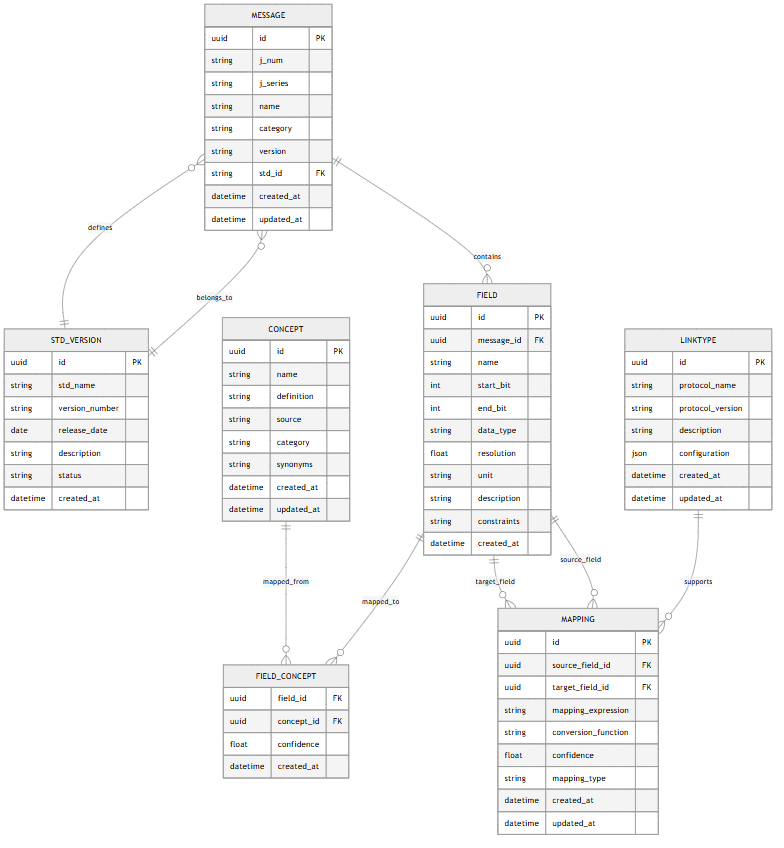
\includegraphics[width=0.9\textwidth]{chapters/fig-0/data_model.png}
    \caption{核心数据模型ER图}
    \label{fig:data_model}
\end{figure}

(1)MESSAGE表:存储消息元信息,包含消息编号、名称、类别、版本等基本信息。该表是系统核心表之一,每个消息具有唯一标识符和版本信息,为战术数据链消息的标准化管理提供数据基础。

(2)FIELD表:存储位段定义及约束信息,包含起始位、结束位、分辨率、取值域等详细信息。该表与MESSAGE表通过外键关联,支持一个消息包含多个字段的复杂结构。

(3)CONCEPT表:存储语义概念库,定义术语与来源信息,为语义互操作提供概念基础。该表支持概念的定义、分类和关系管理,构建完整的语义概念体系。

(4)MAPPING表:存储跨标准映射规则,包含表达式、转换函数、置信度等信息。该表支持不同标准间的字段映射和转换规则定义,为语义互操作提供精确的转换机制。

(5)STD\_VERSION表:存储标准版本管理信息,记录标准的版本号、发布日期、修订历史等关键信息。该表为多标准版本管理提供完整的版本控制机制。

(6)LINKTYPE表:存储协议类型定义与配置信息,支持不同数据链协议的配置和管理。该表为多协议支持提供灵活的配置机制。

\subsection{约束与索引设计}

数据库设计采用严格的约束和高效的索引策略,确保数据完整性和查询性能,构建了完善的数据管理机制。

主外键设计采用UUID主键与业务唯一约束相结合的设计方案。UUID主键确保全局唯一性,避免分布式环境下的主键冲突问题;业务唯一约束(如MESSAGE(j\_num, std\_id))保证业务逻辑的正确性。

完整性约束实现位段检查(start\_bit < end\_bit)、置信度范围(0–1)等多种约束机制。这些约束通过数据库的CHECK约束实现,在数据层面确保数据的有效性,防止无效数据的入库。

索引策略设计组合索引(std\_id, j\_series, j\_num)和全文索引(概念模糊检索)等多种索引类型。组合索引支持多条件查询,提升复杂查询的性能;全文索引支持语义概念的模糊检索。

性能优化采用分区表与缓存机制相结合的策略。对于大数据量表,使用分区策略减少查询范围,通过水平分区和垂直分区相结合的方式提升查询效率;对于热点数据,使用Redis缓存提升访问速度。

\subsection{微服务数据库分离与一致性}

各微服务采用独立的数据库设计,通过多种机制保证数据一致性,构建了完善的分布式数据管理体系。

数据库分离要求每个微服务拥有独立的数据库,避免数据耦合和单点故障问题。这种设计提高系统的可扩展性和容错能力,使得各个服务能够独立演进和部署。

一致性机制采用Saga模式与事件驱动同步机制相结合的方式实现最终一致性。Saga模式将复杂的分布式事务分解为多个本地事务,通过补偿操作保证数据一致性,解决分布式环境下的数据一致性问题。

数据同步通过CDC(Change Data Capture)机制捕获变更事件,实现数据的实时同步。CDC机制精确捕获数据库的变更操作,将变更事件发送到消息队列,为数据同步提供可靠的技术保障。

跨服务同步借助消息队列实现跨服务数据同步。当某个服务的数据发生变化时,系统通过消息队列通知其他相关服务进行数据更新,形成松耦合的数据同步机制。

\section{跨数据链协议互操作架构设计}

\subsection{多协议支持体系}

系统支持多种数据链协议,包括MIL-STD-6016、MAVLink、MQTT、Link 16等,构建了四层互操作体系架构,如图\ref{fig:multi_protocol_support}所示:

\begin{figure}[H]
    \centering
    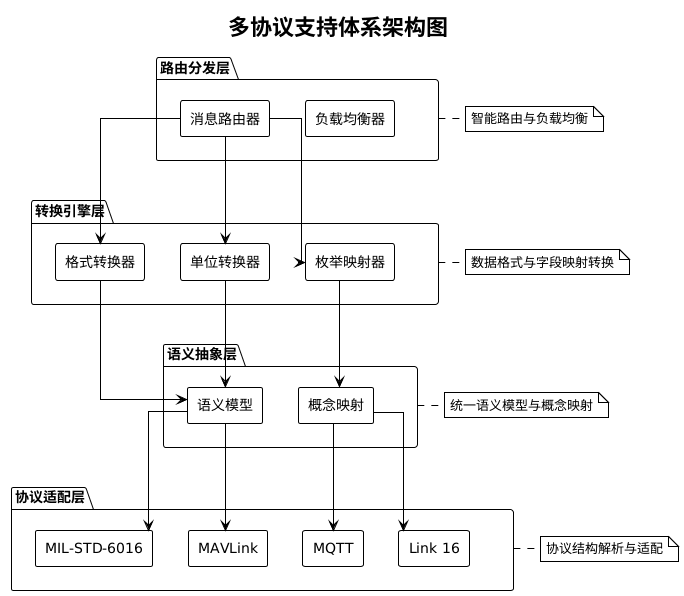
\includegraphics[width=0.9\textwidth]{chapters/fig-0/multi_protocol_support_simple.png}
    \caption{多协议支持体系架构图}
    \label{fig:multi_protocol_support}
\end{figure}

协议适配层作为互操作体系的基础层,负责对各链路标准的结构解析与适配。该层解析不同协议的消息格式,提取字段信息,转换为统一的内部表示,为上层处理提供标准化的数据接口。

语义抽象层建立统一的语义模型与概念映射机制,将不同协议中的概念映射到统一的概念空间。该层通过语义建模技术,实现跨协议的概念对齐和语义理解,为协议间的语义互操作提供概念基础。

转换引擎层实现协议到协议的数据格式与字段映射转换功能,包括格式转换、单位转换、枚举映射等多种转换操作。该层提供灵活的转换规则配置机制,支持复杂的数据转换需求。

路由分发层负责消息智能路由与负载均衡,将消息路由到正确的目标协议,实现负载均衡和故障转移。该层通过智能路由算法,优化消息传输路径,提高系统的整体性能和可靠性。

\subsection{CDM四层法语义互操作模型}

基于"Common Data Model (CDM)"四层方法,系统实现了协议级语义对齐,构建了完整的语义互操作体系,如图\ref{fig:cdm_four_layer}所示:

\begin{figure}[H]
    \centering
    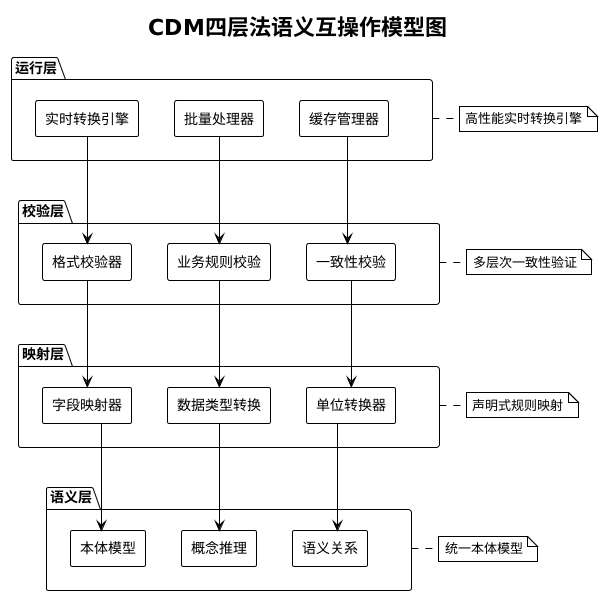
\includegraphics[width=0.9\textwidth]{chapters/fig-0/cdm_four_layer_simple.png}
    \caption{CDM四层法语义互操作模型图}
    \label{fig:cdm_four_layer}
\end{figure}

语义层作为CDM四层方法的基础层,建立统一的本体模型和概念推理机制。该层通过本体技术构建统一的概念模型,支持概念的定义、分类和推理,使系统能够深入理解概念间的语义关系。

映射层采用声明式规则映射和YAML配置化管理方式,使用YAML配置文件定义映射规则,支持规则的版本管理和动态更新。映射规则涵盖字段映射、数据类型转换、单位转换等多种转换需求。

校验层提供多层次的一致性验证和金标准回归测试机制,包括格式校验、业务规则校验、一致性校验等多种校验方式。金标准回归测试确保转换结果的准确性,为语义互操作的质量提供可靠保障。

运行层实现高性能实时转换引擎,采用高效的转换算法支持实时消息转换和批量处理。该层通过缓存和优化技术,提供高性能的转换服务,满足战术数据链对实时性和性能的严格要求。

\subsection{语义互操作系统组成}

系统包含四个核心组件,实现从概念级到消息级的自动语义互操作,构建了完整的语义互操作处理体系,如图\ref{fig:semantic_interop_system}所示:

\begin{figure}[H]
    \centering
    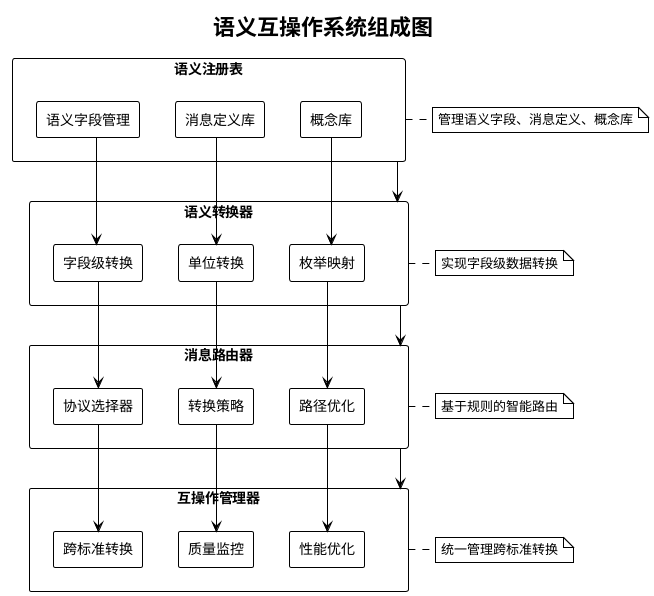
\includegraphics[width=0.9\textwidth]{chapters/fig-0/semantic_interop_system_simple.png}
    \caption{语义互操作系统组成图}
    \label{fig:semantic_interop_system}
\end{figure}

语义注册表作为系统的核心组件之一,负责管理语义字段、消息定义、概念库等核心信息。该组件提供语义信息的注册、查询和更新功能,支持语义概念的版本管理,为语义互操作提供统一的信息管理平台。

语义转换器实现字段级数据转换、单位转换、枚举映射等关键功能,该组件支持多种转换算法,包括数值转换、字符串转换、枚举映射等。通过灵活的转换规则配置,该组件能够处理复杂的跨协议数据转换需求。

消息路由器基于规则的智能路由机制,实现协议选择和转换策略的自动优化。该组件根据消息类型、源协议、目标协议等信息,自动选择最优的转换策略,通过智能路由算法优化消息传输路径。

互操作管理器统一管理跨标准转换、质量监控、性能优化等关键功能,该组件提供转换过程的监控和管理功能,包括性能统计、错误处理、质量评估等。通过全方位的管理机制,该组件确保语义互操作过程的稳定性和高效性。

\subsection{数据一致性与冲突解决}

系统采用多种机制保证跨链路数据的一致性和冲突解决,构建了完善的数据质量管理体系。

一致性协议采用最终一致性协议与版本号优先策略相结合的方式。对于非关键数据,使用最终一致性协议,在保证系统性能的同时确保数据的最终一致性;对于关键数据,使用强一致性保证,确保数据的实时一致性。

冲突解决实现时间戳优先、版本号优先、人工仲裁等多种策略。当数据发生冲突时,系统根据预定义的策略自动解决冲突,通过智能冲突检测和解决算法,最大程度地减少数据冲突的影响;必要时提供人工干预机制,确保复杂冲突情况下的数据正确性。

数据校验提供格式验证、规则校验、完整性验证等多层次校验机制。每个转换过程都经过严格的校验,确保数据的正确性和完整性,通过多层次的校验体系,有效防止错误数据的传播。

质量保障实现跨链路数据同步质量监控,持续监控数据转换的质量,包括准确率、完整性、一致性等关键指标。通过实时质量监控和预警机制,系统能够及时发现和解决数据质量问题。

\section{自动化信息标准导入架构设计}

\subsection{标准化导入流程}

自动化导入系统实现从PDF/Excel/XML等标准文档到数据库的全流程自动处理,如图\ref{fig:import_pipeline}所示:

\begin{figure}[H]
    \centering
    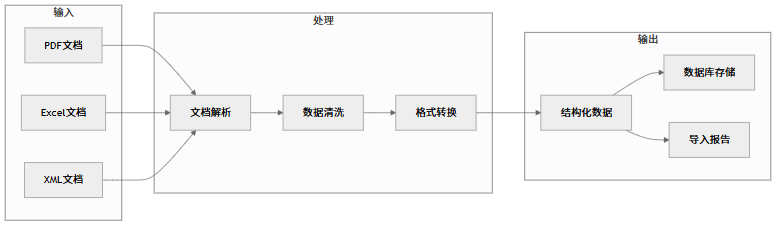
\includegraphics[width=0.9\textwidth]{chapters/fig-0/import_pipeline_simple.png}
    \caption{自动化导入流程}
    \label{fig:import_pipeline}
\end{figure}

处理流程包括PDF文档解析、文本提取、表格识别、字段解析、数据清洗、结构化导入、校验报告生成等关键步骤。每个步骤都经过严格的验证和质量控制,确保导入数据的准确性和完整性。

文档解析阶段使用OCR技术和PDF解析库提取文档中的文本和表格信息。对于扫描文档,使用Tesseract OCR进行文字识别,支持多语言文字识别;对于文本型PDF,直接提取文本内容,通过多种解析技术的结合,确保不同类型文档的准确解析。

结构化处理阶段将提取的文本信息转换为结构化的数据格式。通过规则匹配和机器学习算法,系统能够智能识别消息定义、字段信息和约束条件,将非结构化的文档内容转换为标准化的数据结构。

数据清洗阶段对提取的数据进行全面的清洗和验证,包括格式检查、完整性验证、一致性检查等多种验证机制。发现的问题会详细记录到错误日志中,供后续处理和分析。

导入存储阶段将清洗后的数据导入到数据库中,并生成详细的导入报告。报告包括成功导入的记录数、失败记录数、错误信息等关键统计信息,为导入过程的质量评估和问题追踪提供完整的记录。

\subsection{关键技术与工具链}

系统采用多种先进的技术和工具,确保导入过程的准确性和效率,构建了完整的技术支撑体系。

文档解析使用PyMuPDF、pdfplumber、Camelot、Tesseract OCR等专业工具。PyMuPDF提供高性能的PDF解析能力,pdfplumber专门用于表格提取,Camelot提供精确的表格识别功能,Tesseract OCR支持多语言文字识别,这些工具的结合使用确保不同类型文档的准确解析。

结构化导入采用Pandas + SQLAlchemy + MySQL技术栈。Pandas提供强大的数据处理能力,支持复杂的数据操作和分析;SQLAlchemy提供ORM支持,简化数据库操作;MySQL提供可靠的数据存储,确保数据的安全性和一致性。

格式识别使用MIME检测与规则匹配技术相结合的方式。MIME检测能够快速识别文件类型,为后续处理提供基础信息;规则匹配提供精确的格式识别和内容解析,通过智能识别算法,确保不同格式文档的准确处理。

校验机制实现自动检测字段重叠、位长一致性、枚举合法性等关键功能。系统能够自动检测数据中的各种问题,并提供修复建议,通过智能校验机制,确保导入数据的质量和准确性。


\subsection{数据清洗与质量保证}

系统提供完善的数据清洗和质量保证机制,构建了全方位的数据质量管理体系。

清洗策略实现空值处理、重复检测、标准一致性校验等关键功能。系统能够自动处理各种数据质量问题,包括缺失值、重复值、格式错误等常见问题,通过智能清洗算法,显著提升数据质量。

质量指标监控数据完整性、语义保持率、转换准确率等关键指标。这些指标能够全面反映数据质量的水平,为质量改进提供科学依据,通过持续的质量监控,系统能够及时发现和解决数据质量问题。

验证机制提供格式验证、业务规则验证、一致性验证等多层次验证体系。每个验证层次都有明确的验证规则和错误处理机制,通过多层次的验证保障,确保数据的准确性和一致性。

错误处理实现异常记录、自动修复、人工审核等完整功能。系统能够自动处理大部分数据问题,对于复杂问题提供人工干预机制,通过智能化的错误处理,最大程度地减少数据质量问题的影响。

\section{微服务通信与运行保障设计}

\subsection{服务通信与安全}

系统采用多种通信模式和安全机制,确保服务间的可靠通信,构建了完善的通信安全保障体系。

同步通信使用REST/gRPC/GraphQL等多种协议进行同步通信。REST API主要用于简单的CRUD操作,提供标准化的HTTP接口;gRPC用于高性能的内部服务通信,充分利用其二进制协议的高效性;GraphQL用于复杂的数据查询,提供灵活的数据获取能力。

异步通信使用RabbitMQ、Redis Pub/Sub进行异步通信。RabbitMQ提供可靠的消息传递和事务支持,确保关键业务数据的可靠传输;Redis Pub/Sub提供高性能的实时通知,支持轻量级消息传递,形成同步与异步相结合的通信机制。

服务发现通过Consul + Kubernetes DNS实现服务的自动发现和负载均衡。服务启动时自动注册到服务发现中心,其他服务通过服务名进行调用,实现服务间的松耦合通信,提高系统的可维护性和可扩展性。

通信安全使用TLS双向认证、服务间认证确保通信安全。所有服务间通信都使用TLS加密,并通过JWT令牌进行身份验证,构建多层次的安全防护体系。

\subsection{分布式数据管理与灾备}

系统采用分布式数据管理策略,确保数据的安全性和可用性,构建了完善的数据保护体系。

数据分离实现数据分离与所有权隔离机制。每个微服务拥有独立的数据存储,有效避免数据耦合和单点故障问题,这种设计显著提高系统的可扩展性和容错能力,为微服务架构的灵活性提供数据层面的支撑。

一致性保证采用Saga与事件溯源相结合的方式保证最终一致性。Saga模式将复杂的分布式事务分解为多个本地事务,通过补偿操作保证数据一致性,有效解决分布式环境下的数据一致性问题。

灾备机制实现多区域备份与灾难恢复机制。系统支持跨区域的数据备份和灾难恢复,确保在重大故障情况下的数据安全,通过完善的灾备体系,最大程度地降低数据丢失的风险。

数据同步通过实时同步、批量同步、增量同步等多种方式实现数据同步。根据数据的重要性和实时性要求,系统能够智能选择合适的同步策略,确保不同场景下的数据同步需求。

\subsection{配置与治理体系}

系统提供完善的配置管理和服务治理机制,构建了全方位的系统管理体系。

配置管理实现集中配置与环境隔离(Consul + ConfigMap)机制。所有配置信息都存储在配置中心,支持动态更新和环境隔离,通过统一的配置管理,确保系统配置的一致性和可维护性,为不同环境的部署提供灵活的配置支持。

监控体系提供全链路监控(Prometheus + Grafana + Jaeger)能力。Prometheus负责指标收集,提供全面的性能监控数据;Grafana提供可视化展示,支持丰富的图表和仪表板;Jaeger提供分布式链路追踪,实现完整的系统监控体系。

日志管理实现结构化日志与追踪链路功能。所有日志都采用结构化格式,支持日志聚合、搜索和分析,通过统一的日志管理,为系统运维和问题排查提供强有力的支撑。

服务治理提供健康检查、故障检测、负载均衡等服务治理功能。系统能够自动检测服务健康状态,并进行故障转移和负载均衡,通过智能化的服务治理,确保系统的稳定性和高可用性。

\subsection{容错与弹性设计}

系统采用多种容错和弹性设计机制,确保在异常情况下的服务可用性,构建了完善的故障处理体系。

容错机制实现熔断、重试、降级机制确保系统在异常情况下保持服务可用。当服务调用失败率达到预设阈值时,系统自动开启熔断器,有效避免级联故障;对于临时性故障,系统自动进行重试操作;当系统负载过高时,系统自动降级到简化功能,确保核心服务的可用性。

弹性伸缩通过Kubernetes HPA实现自动伸缩与资源弹性分配。系统根据CPU、内存使用率和自定义指标,自动调整服务实例数量,实现资源的动态优化配置,确保系统在不同负载情况下的高效运行。

故障恢复提供自动恢复、手动干预、数据修复等完整功能。系统能够自动处理大部分故障,对于复杂故障提供人工干预机制,通过智能化的故障处理,最大程度地减少故障对系统的影响。

性能保障确保响应时间保证、吞吐量稳定、故障恢复能力。系统通过多种优化技术,提供高性能和稳定的服务,满足战术数据链对系统性能和可靠性的严格要求。

通过微服务架构与跨数据链协议互操作系统的设计,本研究构建了功能完整、性能优异、可扩展性强的战术数据链信息标准处理平台。该平台支持多种数据链协议的语义互操作,具备自动化导入、智能转换、质量保证等先进功能,为战术数据链的标准化和互操作提供技术基础。